\section{Results}
\label{sec:results}

\subsection{The truth and the precision of the measurement}
\label{sec:res-truth}

The true 99.9 percent quantile of the annual loss grows from EUR \truthA{} million at $\xi=\xiA{}$ to EUR \truthB{}, \truthC{} and \truthD{} million at 0.8, 0.96 and 1.1, a factor of about 60 for a change of the tail index of 0.5 (\cref{tab:truth}). The three computations of the truth agree: the Panjer value differs from the Fourier value by at most \panGapD{} percent and the Monte Carlo of ten million years lies within three standard errors of it in every variant.
The measurement is itself an estimate over a finite number of histories. \Cref{fig:precision} shows the relative standard deviation of the interquartile range over random subsets of the histories of a cell, median over the cells: for the splice it is \subSpFifty{} percent with 50 histories, \subSpHundred{} percent with 100, \subSpTwoFifty{} percent with 250 and \subSpFiveHundred{} percent with 500, and for the single loss approximation \subSlFifty{}, \subSlHundred{}, \subSlTwoFifty{} and \subSlFiveHundred{} percent.
The curves follow the $n^{-1/2}$ reference, so the 1{,}000 histories of a cell give the interquartile range of the splice to a relative standard deviation of about five percent (\subSpFiveHundred{} percent at 500 histories divided by $\sqrt2$), which the intervals of \cref{tab:main-results} reflect.

\begin{figure}[htbp]
\centering
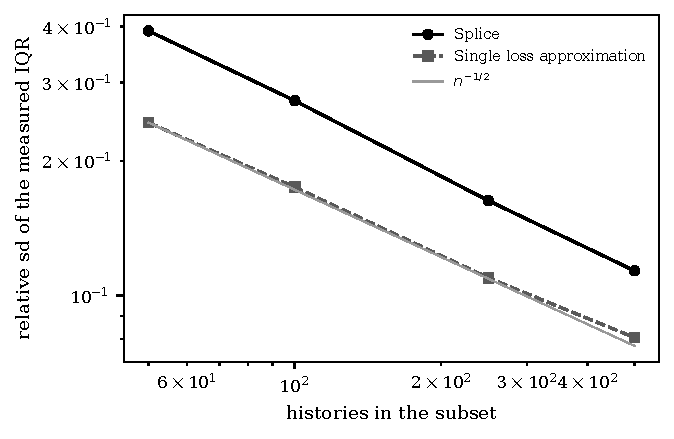
\includegraphics[width=0.62\textwidth]{precision-vs-histories.pdf}
\caption{Relative standard deviation of the measured interquartile range of the capital ratio over 400 random subsets of 50 to 500 of the 1{,}000 histories of a cell, median over the 16 cells, for the splice and the single loss approximation; the grey line is the $n^{-1/2}$ reference scaled to the first point.}
\label{fig:precision}
\end{figure}

\subsection{The main comparison}
\label{sec:res-main}

\Cref{tab:main-results} gives, for each of the 16 cells, the splice and the single loss approximation as multiples of the true quantile, with 95 percent bootstrap intervals over the 1{,}000 histories. The splice is defined on \cSpDTaNdef{} to \cSpATaNdef{} of the 1{,}000 histories of a cell, and \cref{fig:iqr-by-cell} plots its interquartile range, with the interval, against the tail index for the four cells. The interquartile range of the splice capital lies between \spIqrMin{} and \spIqrMax{} times the true quantile:
the smallest value is at $\xi=0.6$ with 10 years and a threshold of EUR 20,000, where the interval is \cSpATbIqrLo{} to \cSpATbIqrHi{}, and the largest is at $\xi=0.96$ with 5 years and EUR 20,000. The same table shows a median ratio between \cSpDFaMed{} and \cSpCTbMed{} for the splice, so the splice both understates the truth in the typical history and disperses by a multiple of it.
For the single loss approximation, which is defined on every history, the interquartile range is between \cSlATaIqr{} and \cSlDFbIqr{}, roughly half of the splice's, and the share of histories below the truth is 50 to 63 percent.

\begin{table}[htbp]
\centering\scriptsize
\caption{The 99.9 percent capital of the lognormal-GPD splice and of the single loss approximation as a multiple of the true quantile, in the 16 cells of 1{,}000 independent histories each: the histories on which the splice is defined, the median ratio, the interquartile range of the ratio with its 95 percent percentile bootstrap interval over the histories (2{,}000 resamples), and the percentage of histories below the truth. The single loss approximation is defined on every history.}
\label{tab:main-results}
\fitwidth{\begin{tabular}{rrrr|rrr|rrr}
\toprule
 & & & \multicolumn{4}{c|}{Splice} & \multicolumn{3}{c}{Single loss approximation} \\
$\xi$ & Years & $H$ (EUR k) & Defined & Median & IQR [95\% CI] & Below 1 (\%) & Median & IQR [95\% CI] & Below 1 (\%) \\
\midrule
0.6 & 5 & 10 & 959 & 0.76 & 1.95 [1.67, 2.29] & 56 & 0.84 & 1.03 [0.96, 1.13] & 58 \\
0.6 & 5 & 20 & 771 & 0.76 & 2.03 [1.68, 2.39] & 58 & 0.84 & 1.10 [1.01, 1.24] & 57 \\
0.6 & 10 & 10 & 996 & 0.85 & 1.43 [1.25, 1.59] & 56 & 0.84 & 0.69 [0.61, 0.76] & 61 \\
0.6 & 10 & 20 & 859 & 0.84 & 1.35 [1.13, 1.61] & 57 & 0.80 & 0.73 [0.67, 0.79] & 63 \\
\midrule
0.8 & 5 & 10 & 904 & 0.66 & 2.74 [2.23, 3.09] & 59 & 0.92 & 1.28 [1.18, 1.44] & 54 \\
0.8 & 5 & 20 & 682 & 0.64 & 2.56 [2.15, 3.42] & 60 & 0.90 & 1.53 [1.38, 1.76] & 54 \\
0.8 & 10 & 10 & 971 & 0.82 & 1.78 [1.54, 2.11] & 55 & 0.93 & 0.82 [0.70, 0.90] & 54 \\
0.8 & 10 & 20 & 727 & 0.91 & 1.98 [1.71, 2.24] & 53 & 0.96 & 1.02 [0.91, 1.14] & 52 \\
\midrule
0.96 & 5 & 10 & 725 & 0.78 & 3.10 [2.29, 3.87] & 57 & 0.94 & 1.34 [1.19, 1.56] & 53 \\
0.96 & 5 & 20 & 550 & 0.63 & 3.30 [2.44, 4.70] & 56 & 0.90 & 1.74 [1.50, 1.94] & 54 \\
0.96 & 10 & 10 & 818 & 0.76 & 2.11 [1.76, 2.54] & 55 & 0.97 & 0.90 [0.78, 0.99] & 52 \\
0.96 & 10 & 20 & 572 & 0.93 & 2.23 [1.83, 2.58] & 53 & 0.97 & 1.18 [1.05, 1.29] & 51 \\
\midrule
1.1 & 5 & 10 & 229 & 0.50 & 3.30 [2.39, 5.26] & 57 & 0.95 & 1.32 [1.18, 1.48] & 52 \\
1.1 & 5 & 20 & 443 & 0.72 & 3.18 [2.56, 4.60] & 55 & 0.84 & 1.78 [1.50, 1.98] & 55 \\
1.1 & 10 & 10 & 128 & 0.89 & 1.68 [1.32, 3.32] & 52 & 0.94 & 0.95 [0.87, 1.03] & 53 \\
1.1 & 10 & 20 & 409 & 0.73 & 2.32 [1.90, 2.78] & 57 & 1.00 & 1.44 [1.29, 1.63] & 50 \\
\bottomrule
\end{tabular}}
\end{table}


\begin{figure}[htbp]
\centering
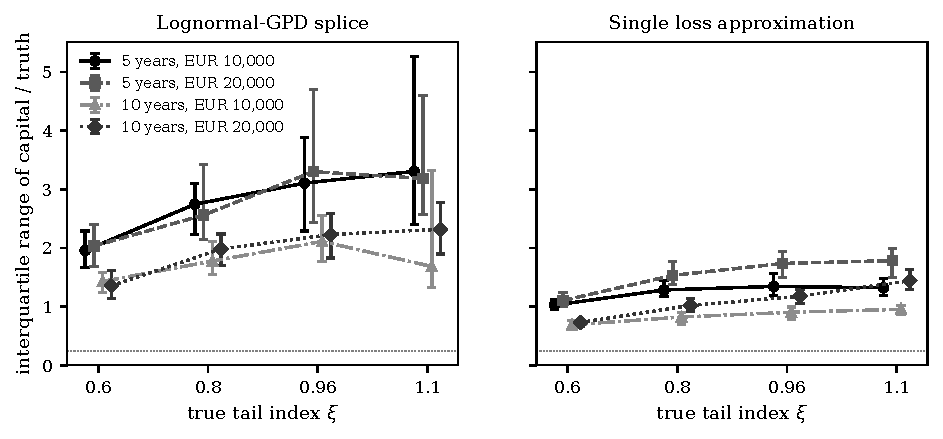
\includegraphics[width=0.95\textwidth]{iqr-by-cell.pdf}
\caption{Interquartile range of the capital divided by the true quantile against the true tail index for the splice (left) and the single loss approximation (right), in the four combinations of history length and collection threshold, with 95 percent bootstrap intervals over 1{,}000 histories; the dotted line is the green limit 0.25 of the product.}
\label{fig:iqr-by-cell}
\end{figure}

\Cref{fig:ecdf} shows the distribution of the ratio itself for four rungs in the cell of 10 years and EUR 20,000. The curves are wide on a logarithmic axis: at $\xi=0.96$ the 5th and the 95th percentiles of the splice ratio are \cSpCTbPlo{} and \cSpCTbPhi{}, a factor of more than one hundred, and the share of histories within a factor of two of the truth is only \plSpWithin{} percent for the splice over all cells, against \plSlWithin{} for the single loss approximation and \plScWithin{} for the scenario combination.

\begin{figure}[htbp]
\centering
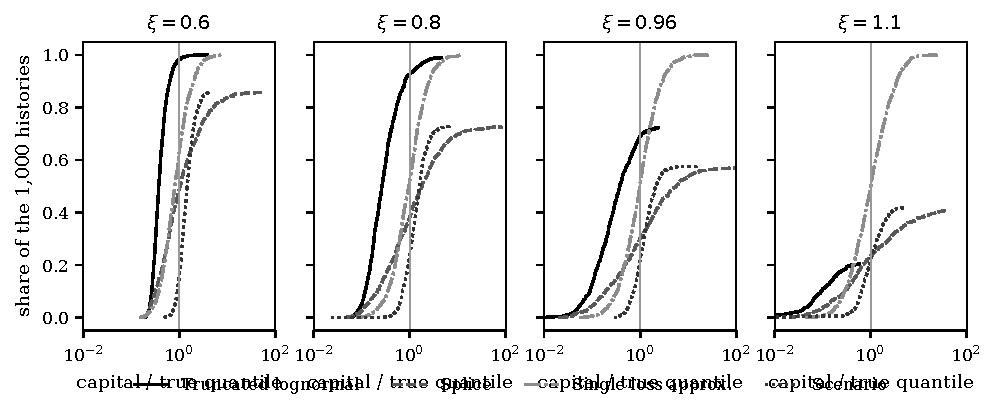
\includegraphics[width=\textwidth]{ecdf-ratio.pdf}
\caption{Cumulative share of the 1{,}000 histories of the cell of 10 years and threshold EUR 20,000 whose capital divided by the true quantile is at most the abscissa, for the truncated lognormal, the splice, the single loss approximation and the scenario combination, at the four tail indices; a curve ends below one where the rung is undefined on the remaining histories, and the vertical line marks the truth.}
\label{fig:ecdf}
\end{figure}

\subsection{The ladder}
\label{sec:res-ladder}

\Cref{tab:rungs} summarises the ten rungs over the 16 cells and \cref{fig:iqr-by-rung} plots their interquartile ranges at the shortest and the longest history. No rung is stable. The lognormal that ignores the threshold has a very small interquartile range, \plLgIqr{} on average, because its error is systematic: its median capital is \cLgATbMed{} of the truth at $\xi=0.6$ and \cLgDTbMed{} at $\xi=1.1$,
and practically no history (\plLgWithin{} percent) falls within a factor of two of the truth. The truncated lognormal removes part of that bias, and is defined on only \plTrDef{} percent of the histories, \cTrDTaNdef{} of the 1{,}000 at $\xi=1.1$ with 10 years and EUR 10,000. The scenario combination has a mean interquartile range of \plScIqr{}, comparable with the mean-adjusted fits (\plMaIqr{}, \plObIqr{} and \plCvIqr{} for the maximum likelihood, bias-robust and Cram\'er-von Mises fits), and the highest share within a factor of two, \plScWithin{} percent, but its prior is the expert's true severity quantile of the generator, rounded to two significant figures, so it measures what an informative prior is worth and not an estimate from data.

\begin{table}[htbp]
\centering\small
\caption{The ten estimation rungs over the 16 cells: the share of the 16{,}000 histories on which the rung returns a capital, the mean over cells of the median ratio to the truth, the range over cells of the interquartile range of the ratio, the share of defined histories within a factor of two of the truth with its Wilson 95 percent interval, and the number of cells on which the capital stability test is red.}
\label{tab:rungs}
\fitwidth{\begin{tabular}{lrrrrr}
\toprule
Rung & Defined (\%) & Mean median & IQR range over cells & Within factor 2 (\%) [95\% CI] & Red cells \\
\midrule
Lognormal, threshold ignored & 100 & 0.06 & 0.00 to 0.03 & 0.0 [0.0, 0.0] & 16 of 16 \\
Truncated lognormal & 74 & 0.20 & 0.05 to 0.35 & 14.8 [14.2, 15.5] & 16 of 16 \\
Lognormal-GPD splice & 67 & 0.76 & 1.35 to 3.30 & 34.0 [33.1, 34.9] & 16 of 16 \\
Single loss approximation & 100 & 0.91 & 0.69 to 1.78 & 57.2 [56.4, 57.9] & 16 of 16 \\
Single loss approximation, mean correction & 66 & 0.85 & 0.56 to 1.32 & 65.5 [64.5, 66.4] & 12 of 12 \\
Scenario combination & 68 & 1.18 & 0.51 to 1.23 & 82.3 [81.6, 83.0] & 16 of 16 \\
\midrule
Mean-adjusted single loss approximation & 71 & 0.70 & 0.12 to 1.31 & 61.6 [60.7, 62.5] & 16 of 16 \\
Cram\'er-von Mises GPD & 70 & 0.65 & 0.13 to 1.85 & 46.8 [45.9, 47.8] & 16 of 16 \\
Optimally bias-robust GPD & 70 & 0.71 & 0.12 to 1.48 & 59.6 [58.7, 60.5] & 16 of 16 \\
Cram\'er-von Mises lognormal & 72 & 0.13 & 0.06 to 0.26 & 8.3 [7.8, 8.8] & 16 of 16 \\
\bottomrule
\end{tabular}}
\end{table}


\begin{figure}[htbp]
\centering
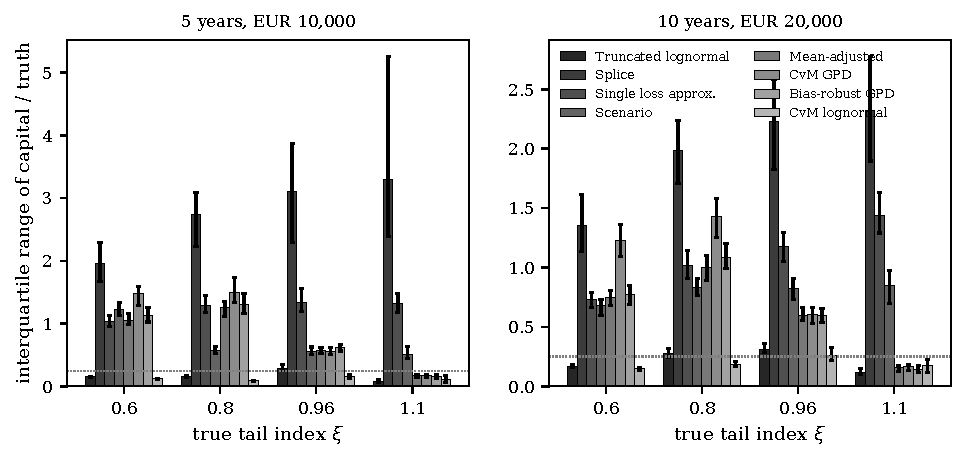
\includegraphics[width=\textwidth]{iqr-by-rung.pdf}
\caption{Interquartile range of the capital divided by the true quantile by estimation rung and tail index, in the cell of 5 years and threshold EUR 10,000 (left) and in the cell of 10 years and threshold EUR 20,000 (right), with 95 percent bootstrap intervals; the dotted line is the green limit 0.25 of the product.}
\label{fig:iqr-by-rung}
\end{figure}

\Cref{tab:lights} counts the lights of the capital stability test: every rung is red in every cell where it is defined, \redTotal{} of \redTotal{} rows, and \redSix{} of \rowsSix{} on the six-rung ladder. The test combines the interquartile range and the bias, so a rung may be red for either reason; the lognormals, which understate the truth by a large margin, fail on bias, and the splice, the single loss approximation and the scenario combination fail on dispersion.

\begin{table}[htbp]
\centering\small
\caption{The lights of the capital stability test over the 16 cells for each rung, against the limits of 0.25 and 0.50 on the interquartile range of the ratio and 0.10 and 0.25 on the absolute bias: the number of cells in which each rung is green, amber and red, from the committed documents. The last row, the mean-corrected single loss approximation, is a comparison only and is in no count of the text; it is computed on 12 cells.}
\label{tab:lights}
\begin{tabular}{lrrr}
\toprule
Rung & Green & Amber & Red \\
\midrule
Lognormal, threshold ignored & 0 & 0 & 16 \\
Truncated lognormal & 0 & 0 & 16 \\
Lognormal-GPD splice & 0 & 0 & 16 \\
Single loss approximation & 0 & 0 & 16 \\
Scenario combination & 0 & 0 & 16 \\
Mean-adjusted single loss approximation & 0 & 0 & 16 \\
Cram\'er-von Mises GPD & 0 & 0 & 16 \\
Optimally bias-robust GPD & 0 & 0 & 16 \\
Cram\'er-von Mises lognormal & 0 & 0 & 16 \\
\midrule
\multicolumn{4}{l}{\emph{Comparison only, in no count of the text (form not confirmed)}} \\
Single loss approximation, mean correction & 0 & 0 & 12 \\
\bottomrule
\end{tabular}
\end{table}


\subsection{Bias}
\label{sec:res-bias}

\Cref{fig:median} plots the median ratio, averaged over the four cells of each tail index. The single loss approximation has a mean median of \plSlMed{}, below one in \slBelowCells{} of the 16 cells, and it approaches one as the tail gets heavier; this follows the gap of the approximation at the true parameters, \slGapA{} percent at $\xi=0.6$ and \slGapD{} percent at $\xi=1.1$ (\cref{sec:theory-conditions}).
The splice has a mean median of \plSpMed{}, further from one at every tail index, and the scenario combination overshoots, with \plScMed{}. The median is a statement about the typical history and says nothing about a single bank, whose ratio is spread as in \cref{fig:ecdf}.

\begin{figure}[htbp]
\centering
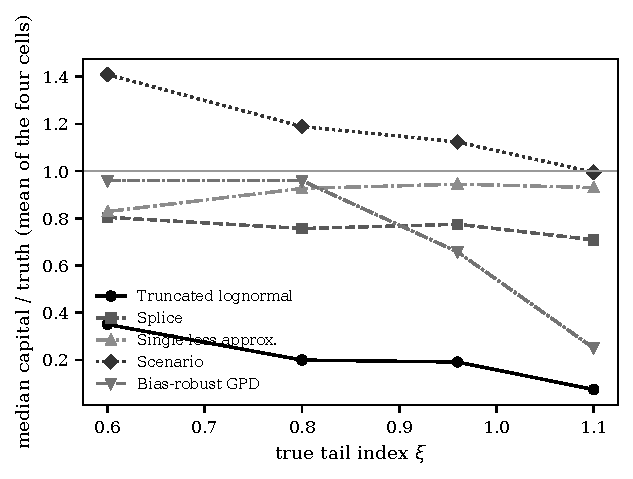
\includegraphics[width=0.62\textwidth]{median-by-xi.pdf}
\caption{Median capital divided by the true quantile against the true tail index for five rungs, averaged over the four cells of each index in which the rung is defined; the horizontal line marks the truth at one.}
\label{fig:median}
\end{figure}

The bias of the splice and of the scenario combination is not a defect of estimation alone. The splice conditions on a fit that succeeds, and the scenario combination takes its tail from the prior, so each has a different relation to the truth than the single loss approximation, whose target is the closed form of the tail.

\subsection{Histories on which a rung is undefined}
\label{sec:res-undefined}

The engine refuses a fit it cannot make, and the refusal is counted. The splice is defined on \plSpDef{} percent of the 16{,}000 histories and the scenario combination on \plScDef{} percent, and the number varies by cell from \cSpDTaNdef{} of 1{,}000 (splice, $\xi=1.1$, 10 years, EUR 10,000) to 996. The truncated lognormal and the splice fail most often where the tail is heaviest, and more often at the lower threshold, because the maximum likelihood fit of a lognormal to Pareto-like data can run to a degenerate maximum.
The statistics of these rungs are conditional on the fit succeeding, and the conditioning flatters them: a history on which the fit fails is exactly one in which the capital would have been furthest from the truth. The single loss approximation is defined on every history and its dispersion is unconditional.

The count of undefined histories is itself a result for a validator. A method that returns a capital on fewer than half of the histories of a bank-like process at the heavy tails cannot be applied to a given bank without a fallback, and a fallback changes the statistics reported here.

\subsection{The wrong conclusion about the mean}
\label{sec:res-mean}

\Cref{tab:tail-index} and \cref{fig:infinite} report the tail index fitted above the collection threshold. At $\xi=0.96$ the share of histories with $\hat\xi\ge1$ is between \infLo{} and \infHi{} percent over the four cells: roughly one history in three concludes that the mean does not exist when it does. At $\xi=1.1$ the share that concludes a finite mean is between \finLo{} and \finHi{} percent.
The median fitted index at $\xi=0.96$ and 5 years is \cXiCFaMed{}, within the error of the true value, so the wrong conclusion is a property of the spread of the fit and not of a bias. Fitting above two, four and eight times the threshold leaves fewer exceedances and moves the share toward one half (columns $2H$ to $8H$ of \cref{tab:tail-index}), which is the behaviour a threshold-stability plot shows and why the plot cannot settle the question at these sample sizes.

\begin{table}[htbp]
\centering\scriptsize
\caption{The tail index fitted above the collection threshold in each cell: the histories with a fit, the median and the 5th to 95th percentiles of the fitted index, the percentage of histories whose index is 1 or more with its Wilson 95 percent interval, the percentage predicted by the normal approximation of the maximum likelihood estimator, and the measured percentage when the fit is made above two, four and eight times the threshold.}
\label{tab:tail-index}
\fitwidth{\begin{tabular}{rrrrrrrrrr}
\toprule
$\xi$ & Years & $H$ (EUR k) & Fits & Median $\hat\xi$ [5\%, 95\%] & $\hat\xi\ge1$ (\%) [95\% CI] & Predicted (\%) & $2H$ & $4H$ & $8H$ \\
\midrule
0.6 & 5 & 10 & 1000 & 0.60 [0.44, 0.75] & 0.0 [0.0, 0.4] & 0.0 & 0 & 0 & 3 \\
0.6 & 5 & 20 & 1000 & 0.59 [0.42, 0.78] & 0.0 [0.0, 0.4] & 0.0 & 0 & 2 & 9 \\
0.6 & 10 & 10 & 1000 & 0.60 [0.48, 0.70] & 0.0 [0.0, 0.4] & 0.0 & 0 & 0 & 0 \\
0.6 & 10 & 20 & 1000 & 0.59 [0.47, 0.73] & 0.0 [0.0, 0.4] & 0.0 & 0 & 0 & 5 \\
\midrule
0.8 & 5 & 10 & 1000 & 0.80 [0.63, 0.96] & 2.4 [1.6, 3.5] & 2.2 & 5 & 12 & 18 \\
0.8 & 5 & 20 & 1000 & 0.79 [0.57, 1.01] & 6.3 [5.0, 8.0] & 5.6 & 11 & 16 & 23 \\
0.8 & 10 & 10 & 1000 & 0.80 [0.69, 0.92] & 0.5 [0.2, 1.2] & 0.2 & 2 & 5 & 11 \\
0.8 & 10 & 20 & 1000 & 0.80 [0.65, 0.94] & 1.2 [0.7, 2.1] & 1.2 & 4 & 9 & 20 \\
\midrule
0.96 & 5 & 10 & 1000 & 0.95 [0.80, 1.13] & 33.2 [30.4, 36.2] & 34.8 & 37 & 38 & 38 \\
0.96 & 5 & 20 & 1000 & 0.95 [0.73, 1.18] & 34.4 [31.5, 37.4] & 38.5 & 37 & 35 & 38 \\
0.96 & 10 & 10 & 1000 & 0.96 [0.84, 1.07] & 26.8 [24.1, 29.6] & 29.0 & 32 & 35 & 36 \\
0.96 & 10 & 20 & 1000 & 0.96 [0.79, 1.12] & 31.7 [28.9, 34.6] & 34.0 & 37 & 40 & 36 \\
\midrule
1.1 & 5 & 10 & 1000 & 1.09 [0.92, 1.26] & 81.8 [79.3, 84.1] & 83.8 & 72 & 66 & 57 \\
1.1 & 5 & 20 & 1000 & 1.08 [0.84, 1.33] & 73.2 [70.4, 75.9] & 75.2 & 64 & 57 & 53 \\
1.1 & 10 & 10 & 1000 & 1.09 [0.98, 1.21] & 91.2 [89.3, 92.8] & 91.8 & 82 & 71 & 66 \\
1.1 & 10 & 20 & 1000 & 1.10 [0.93, 1.27] & 83.6 [81.2, 85.8] & 83.3 & 76 & 67 & 59 \\
\bottomrule
\end{tabular}}
\end{table}


\begin{figure}[htbp]
\centering
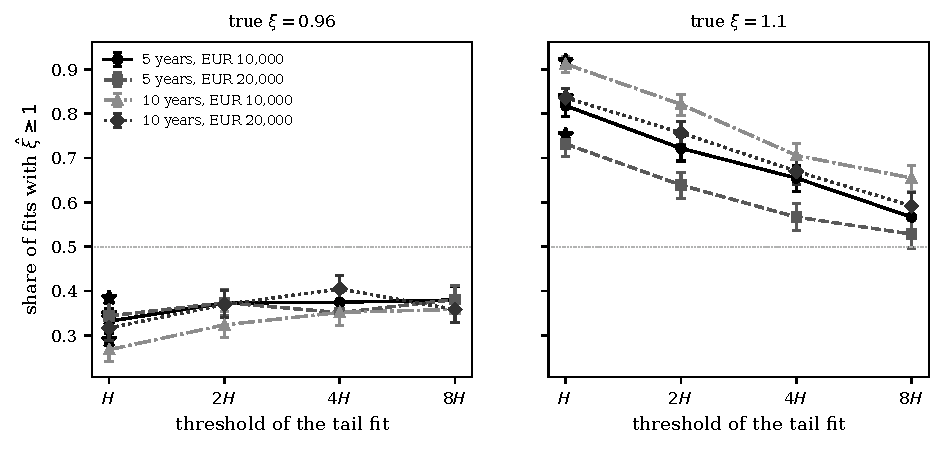
\includegraphics[width=0.95\textwidth]{infinite-mean-share.pdf}
\caption{Share of histories whose fitted tail index is one or more against the threshold of the tail fit, from the collection threshold $H$ to eight times it, for true tail indices 0.96 (left) and 1.1 (right) in the four cells, with Wilson 95 percent intervals; stars mark the share predicted at $H$ by the normal approximation of the theory.}
\label{fig:infinite}
\end{figure}

In no cell of the design is the share of false infinite-mean conclusions at 0.96 below \infLo{} percent, so there is no combination of the lengths and thresholds studied in which a validator can rule out the wrong side of the boundary.

\subsection{The theory against the measurement}
\label{sec:res-theory}

\Cref{tab:theory} and \cref{fig:theory} set the delta-method dispersion of \cref{eq:dispersion} against the measured standard deviation of the logarithm of the ratio of the single loss approximation. The prediction is within \thSdMaxErr{} percent in every cell and its mean error over cells is \thSdMeanErr{} percent, well inside the tolerance of \preSd{} percent of H5.
The interquartile range predicted from the lognormal approximation of the ratio is less accurate: it exceeds the measured one in \thIqrOver{} of the 16 cells, by \thIqrMean{} percent on average and up to \thIqrMaxErr{} percent, because the distribution of the logarithm of the ratio is more peaked than a normal one. The share of histories with $\hat\xi\ge1$ predicted by \cref{eq:misclassification} is within \thShareMaxErr{} points of the measured share in the cells at 0.96 and 1.1, inside the tolerance of \preShare{} points of H6, and it is slightly above the measured share in most cells, as the right panel of \cref{fig:theory} shows.
The same formula gives the history that would bring the interquartile range to 0.25 (\cref{fig:years}): \yrsMin{} years at the lightest tail and shortest threshold and \yrsMax{} years at $\xi=1.1$ with a threshold of EUR 20,000, an order of magnitude more than the 5 or 10 years of a bank.

\begin{table}[htbp]
\centering\scriptsize
\caption{The dispersion of the single loss approximation predicted by the delta method at the true parameters against the dispersion measured over the 1{,}000 histories of each cell: the expected number of recorded losses $k$, the standard deviation of the logarithm of the ratio, measured and predicted, the relative error of the prediction in percent, the interquartile range of the ratio, measured and predicted by a lognormal of the predicted dispersion, and the years of history at which the predicted interquartile range reaches 0.25.}
\label{tab:theory}
\fitwidth{\begin{tabular}{rrrrrrrrrr}
\toprule
$\xi$ & Years & $H$ (EUR k) & $k$ & $\mathrm{sd}$ measured & $\mathrm{sd}$ predicted & Error (\%) & IQR measured & IQR predicted & Years for 0.25 \\
\midrule
0.6 & 5 & 10 & 296 & 0.810 & 0.815 & +0.7 & 1.03 & 1.16 & 97 \\
0.6 & 5 & 20 & 205 & 0.939 & 0.939 & +0.0 & 1.10 & 1.35 & 129 \\
0.6 & 10 & 10 & 592 & 0.596 & 0.577 & -3.2 & 0.69 & 0.80 & 97 \\
0.6 & 10 & 20 & 410 & 0.645 & 0.664 & +3.0 & 0.73 & 0.93 & 129 \\
\midrule
0.8 & 5 & 10 & 326 & 0.954 & 0.930 & -2.5 & 1.28 & 1.34 & 127 \\
0.8 & 5 & 20 & 205 & 1.171 & 1.116 & -4.7 & 1.53 & 1.65 & 182 \\
0.8 & 10 & 10 & 653 & 0.644 & 0.658 & +2.1 & 0.82 & 0.92 & 127 \\
0.8 & 10 & 20 & 410 & 0.791 & 0.789 & -0.3 & 1.02 & 1.11 & 182 \\
\midrule
0.96 & 5 & 10 & 367 & 0.995 & 0.993 & -0.2 & 1.34 & 1.44 & 144 \\
0.96 & 5 & 20 & 205 & 1.241 & 1.249 & +0.6 & 1.74 & 1.89 & 228 \\
0.96 & 10 & 10 & 734 & 0.691 & 0.702 & +1.6 & 0.90 & 0.98 & 144 \\
0.96 & 10 & 20 & 410 & 0.871 & 0.883 & +1.4 & 1.18 & 1.26 & 228 \\
\midrule
1.1 & 5 & 10 & 429 & 1.016 & 1.017 & +0.1 & 1.32 & 1.48 & 151 \\
1.1 & 5 & 20 & 205 & 1.355 & 1.363 & +0.6 & 1.78 & 2.11 & 272 \\
1.1 & 10 & 10 & 857 & 0.716 & 0.719 & +0.5 & 0.95 & 1.01 & 151 \\
1.1 & 10 & 20 & 410 & 0.955 & 0.963 & +0.9 & 1.44 & 1.39 & 272 \\
\bottomrule
\end{tabular}}
\end{table}


\begin{figure}[htbp]
\centering
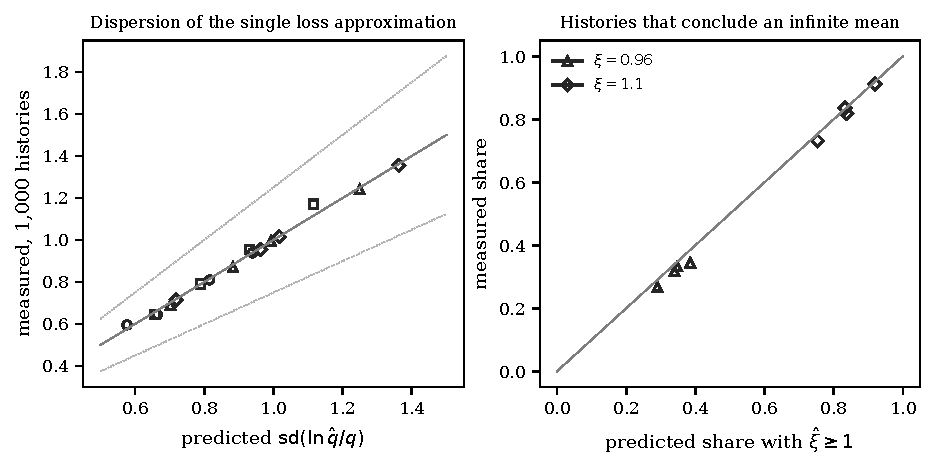
\includegraphics[width=0.95\textwidth]{theory-vs-measured.pdf}
\caption{Measured against predicted standard deviation of the logarithm of the capital ratio of the single loss approximation in the 16 cells, with lines at equality and at plus and minus 25 percent (left), and measured against predicted share of histories with a fitted tail index of one or more at indices 0.96 and 1.1 (right).}
\label{fig:theory}
\end{figure}

\begin{figure}[htbp]
\centering
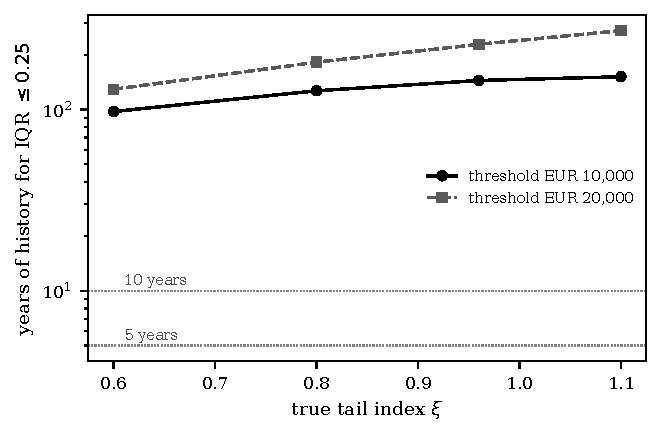
\includegraphics[width=0.62\textwidth]{years-for-green.pdf}
\caption{Years of history at which the predicted interquartile range of the single loss approximation reaches the green limit 0.25 of the product, against the true tail index for the two collection thresholds, on a logarithmic axis; the dotted lines mark the 5 and 10 years of the experiment.}
\label{fig:years}
\end{figure}

\subsection{The standardised approach}
\label{sec:res-sma}

\Cref{tab:sma} gives the capital of the standardised approach as a multiple of the true quantile. It is stable across histories relative to its own level, because it depends on the losses only through the average annual loss and enters the multiplier with the exponent 0.8, and it does not track the tail: its median is \smaA{} times the true quantile at $\xi=0.6$, \smaB{} at 0.8, \smaC{} at 0.96 and \smaD{} at 1.1 in the cell of 10 years and EUR 20,000.
The approach is not calibrated to the 99.9 percent quantile of any bank, so the ratio is a comparison and not an error; it shows that the standardised capital is neither a conservative nor an aggressive proxy for the quantile of this process, but a quantity that does not move with the tail that the quantile follows.

\begin{table}[htbp]
\centering\small
\caption{The standardised approach against the true quantile in the 16 cells: the median over the 1{,}000 histories of the operational risk capital divided by the true 99.9 percent quantile, its first and third quartiles, its interquartile range and the median capital in EUR million, at the business indicator component of EUR 180 million of the synthetic bank.}
\label{tab:sma}
\begin{tabular}{rrrrrrr}
\toprule
$\xi$ & Years & $H$ (EUR k) & Median ratio & Quartiles & IQR & Median capital (EUR m) \\
\midrule
0.6 & 5 & 10 & 4.022 & 3.941 to 4.120 & 0.179 & 136.3 \\
0.6 & 5 & 20 & 3.967 & 3.890 to 4.073 & 0.183 & 134.5 \\
0.6 & 10 & 10 & 4.030 & 3.967 to 4.111 & 0.144 & 136.6 \\
0.6 & 10 & 20 & 3.975 & 3.906 to 4.053 & 0.147 & 134.7 \\
\midrule
0.8 & 5 & 10 & 0.873 & 0.846 to 0.921 & 0.075 & 142.7 \\
0.8 & 5 & 20 & 0.859 & 0.829 to 0.901 & 0.071 & 140.4 \\
0.8 & 10 & 10 & 0.882 & 0.857 to 0.915 & 0.058 & 144.1 \\
0.8 & 10 & 20 & 0.869 & 0.843 to 0.908 & 0.064 & 142.0 \\
\midrule
0.96 & 5 & 10 & 0.239 & 0.227 to 0.258 & 0.031 & 151.6 \\
0.96 & 5 & 20 & 0.233 & 0.221 to 0.254 & 0.033 & 147.7 \\
0.96 & 10 & 10 & 0.242 & 0.231 to 0.261 & 0.030 & 153.6 \\
0.96 & 10 & 20 & 0.239 & 0.227 to 0.258 & 0.031 & 151.6 \\
\midrule
1.1 & 5 & 10 & 0.076 & 0.070 to 0.085 & 0.015 & 162.4 \\
1.1 & 5 & 20 & 0.074 & 0.068 to 0.083 & 0.015 & 158.5 \\
1.1 & 10 & 10 & 0.078 & 0.072 to 0.088 & 0.016 & 167.2 \\
1.1 & 10 & 20 & 0.077 & 0.071 to 0.087 & 0.016 & 165.0 \\
\bottomrule
\end{tabular}
\end{table}


\subsection{Whether each hypothesis held}
\label{sec:res-hypotheses}

\Cref{tab:hypotheses} lists the six predictions of \cref{sec:ed-hypotheses} with the measured values. All six held. H1 holds at two decimals, with a range of \spIqrMin{} to \spIqrMax{}; the bootstrap interval of the smallest cell, \cSpATbIqrLo{} to \cSpATbIqrHi{}, shows that the endpoints of the range are themselves uncertain by tenths of the truth. H2 holds on the six-rung ladder and on the four additional rungs.
H3 and H4 hold with the ranges \infLo{} to \infHi{} and \finLo{} to \finHi{} percent, which round to the stated 27 to 34 and 9 to 27 at the whole percent. H5 and H6 hold with the errors in the table. The agreement of the delta-method dispersion with the measurement is closer than the sampling noise of the measurement in several cells, so the data cannot separate the prediction from a slightly different formula; the evidence is that the formula is adequate for the purpose of finding the history needed, not that it is exact.

\begin{table}[htbp]
\centering\small
\caption{The six predictions stated before the measurements, the value measured on the 16{,}000 histories, and whether each held. H1 to H4 are the quantitative statements of the measurement; H5 and H6 are the predictions of the theory, with the tolerances fixed before they were compared with the 16 cells.}
\label{tab:hypotheses}
\begin{tabularx}{\textwidth}{lXXl}
\toprule
Id & Prediction & Measured & Outcome \\
\midrule
H1 & The interquartile range of the splice capital over the true quantile lies between 1.35 and 3.30 in the 16 cells & 1.3536 to 3.3038 & Held \\
H2 & Every capital stability row of the six-rung ladder is red & 92 of 92 rows red (156 of 156 with the four robust rungs) & Held \\
H3 & 27 to 34 percent (whole percent) of the histories at $\xi=0.96$ conclude an infinite mean & 26.8 to 34.4 percent & Held \\
H4 & 9 to 27 percent (whole percent) of the histories at $\xi=1.1$ conclude a finite mean & 8.8 to 26.8 percent & Held \\
H5 & The delta-method dispersion of the single loss approximation is within 25 percent of the measured one in every cell & largest relative error 4.7 percent & Held \\
H6 & The predicted share of histories with $\hat\xi\ge1$ is within 5 points of the measured one in every cell at $\xi=0.96$ and $1.1$ & largest absolute error 4.1 points & Held \\
\bottomrule
\end{tabularx}
\end{table}

